\documentclass[aspectratio=169]{beamer}

% Egocentric-10K event logs: high-level presentation of the paper.

\usetheme{Madrid}
\usecolortheme{seahorse}
\usepackage{tikz}
\usetikzlibrary{positioning,fit,backgrounds,arrows.meta,calc}
\usepackage{booktabs}
\usepackage{pgfplots}
\pgfplotsset{compat=1.16}

\definecolor{egoblue}{HTML}{2A78D6}
\definecolor{egogreen}{HTML}{1BAF7A}
\definecolor{egoamber}{HTML}{D97E22}
\definecolor{egoplum}{HTML}{8E5BC0}

\setbeamercolor{structure}{fg=egoblue}
\setbeamercolor{frametitle}{bg=egoblue!12, fg=egoblue!50!black}
\setbeamertemplate{navigation symbols}{}
\setbeamertemplate{itemize items}[circle]

\newcommand{\keyc}[1]{\textbf{\textcolor{egoblue}{#1}}}
\newcommand{\keyg}[1]{\textbf{\textcolor{egogreen!70!black}{#1}}}
\newcommand{\keya}[1]{\textbf{\textcolor{egoamber!85!black}{#1}}}

\tikzset{
  iob/.style={draw=black!55, fill=black!4, rounded corners=2.5pt, align=center,
    inner sep=4pt, minimum height=9mm, font=\small},
  mmb/.style={draw=egoblue!75!black, fill=egoblue!10, rounded corners=2.5pt,
    align=center, inner sep=4pt, minimum height=9mm, font=\small},
  txb/.style={draw=egoplum!75!black, fill=egoplum!10, rounded corners=2.5pt,
    align=center, inner sep=4pt, minimum height=9mm, font=\small},
  outb/.style={draw=egogreen!70!black, fill=egogreen!12, rounded corners=2.5pt,
    align=center, inner sep=4pt, minimum height=9mm, font=\small},
  flow/.style={-{Stealth[length=2.2mm]}, line width=0.9pt, draw=black!60},
  flab/.style={font=\scriptsize, text=black!60, align=center},
  stbg/.style={rounded corners=5pt, inner sep=2.5mm},
  stlab/.style={font=\scriptsize\itshape, inner sep=1.5pt},
}

\title[Egocentric Event Logs]{\textbf{Seeing the Process Through the Worker's Eyes}}
\subtitle{Event Logs from Egocentric Factory Videos}
\author[Berti, van der Aalst]{Alessandro Berti \and Wil M.P. van der Aalst}
\institute[PADS, RWTH]{Process and Data Science (PADS), RWTH Aachen University}
\date{2026}

\begin{document}

% ---------------------------------------------------------------- 1
\begin{frame}
  \titlepage
\end{frame}

% ---------------------------------------------------------------- 2
\begin{frame}{The Problem}
  \begin{itemize}\setlength{\itemsep}{9pt}
    \item Process mining needs \keyc{event logs} extracted from information systems
    \item \keya{Manual shop-floor work} leaves few digital traces:
      picking a part, loading a blank into a die, carrying a tray
    \item At best, an MES logs order- or machine-level checkpoints;
      the \keya{actual work} (sequence, duration, interruptions, handling
      overhead) stays \keya{invisible}
  \end{itemize}
  \vspace{5mm}
  \begin{block}{}
    \centering The manual shop floor is a \keya{blind spot} of process mining,
    yet a large share of \keyg{value creation} still happens there.
  \end{block}
\end{frame}

% ---------------------------------------------------------------- 3
\begin{frame}{A New Data Source: Egocentric Video}
  \begin{columns}[T]
  \begin{column}{0.5\textwidth}
    \vspace{2mm}
    \begin{itemize}\setlength{\itemsep}{8pt}
      \item \keyc{Head-mounted cameras} record the shop floor from the
        \keyc{worker's perspective}
      \item Captures hand-object interaction, machine operation, movement
        \keyg{across stations}
      \item \keyc{Egocentric-10K}: thousands of hours of first-person factory
        footage, over 2{,}000 workers, real facilities
    \end{itemize}
    \vspace{3mm}
    \begin{block}{}
      \centering But \keya{raw video is not event data}: no labels,
      no timestamps, no cases.
    \end{block}
  \end{column}
  \begin{column}{0.46\textwidth}
    \begin{center}
      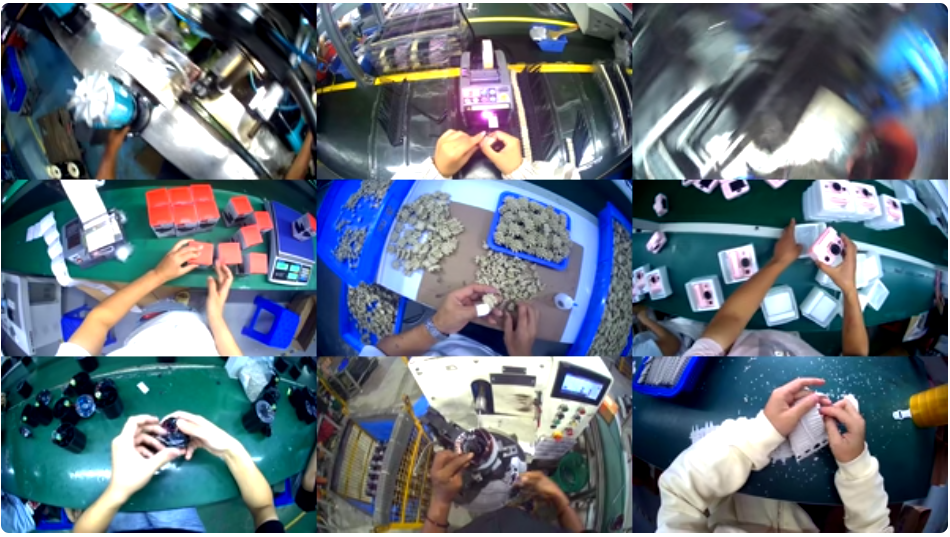
\includegraphics[width=\linewidth]{egocentric10k.png}\\[1mm]
      {\scriptsize Frames from Egocentric-10K}
    \end{center}
  \end{column}
  \end{columns}
\end{frame}

% ---------------------------------------------------------------- 4
\begin{frame}{The Goal}
  \begin{block}{From raw footage to standard event logs, fully automated}
    A \keyc{five-stage pipeline} built only on \keyc{foundation models}
    turns egocentric factory videos into event logs:
    \keya{no task-specific training, no human annotation}.
  \end{block}
  \vspace{4mm}
  \begin{itemize}\setlength{\itemsep}{7pt}
    \item \keyc{RQ1 (feasibility and validity)}: can such a pipeline produce
      \keyg{structurally valid} logs at the scale of hundreds of videos?
    \item \keyc{RQ2 (fidelity)}: how \keyg{faithfully} do the events reflect
      the observed work, temporally and semantically?
    \item \keyc{RQ3 (value)}: which \keyg{analyses} do the logs enable,
      and where do they hit the limits of the data?
  \end{itemize}
  \vspace{3mm}
  \small The logs are \keya{inferred observational data}, not ground truth.
\end{frame}

% ---------------------------------------------------------------- 5
\begin{frame}{The Approach at a Glance}
  \begin{center}
  \resizebox{0.99\textwidth}{!}{%
  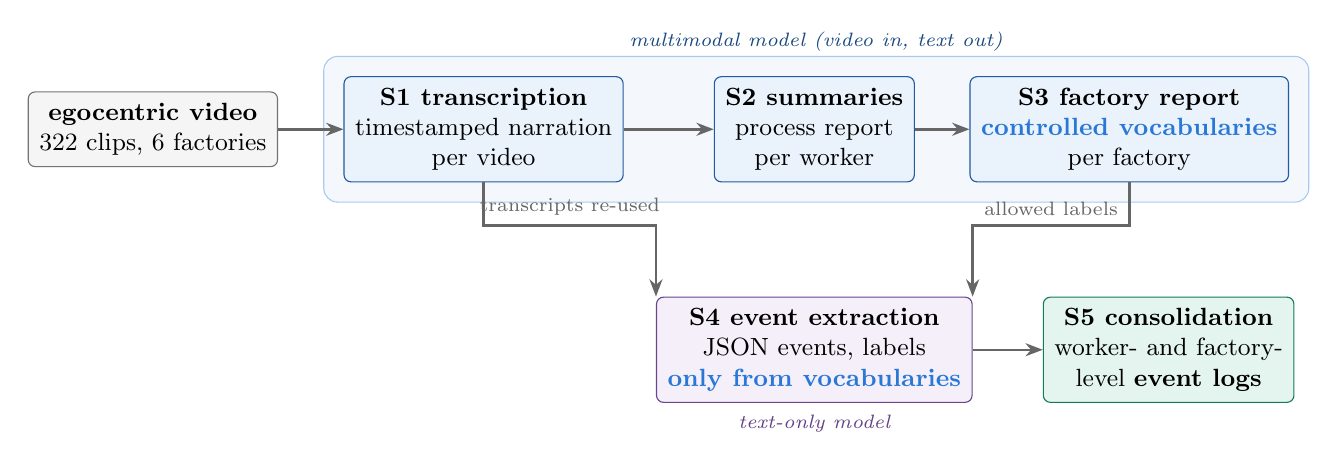
\begin{tikzpicture}[font=\small]
    % inputs
    \node[iob, minimum width=22mm] (vid) at (0,1.5) {\textbf{egocentric video}\\322 clips, 6 factories};
    % multimodal stages
    \node[mmb, minimum width=27mm] (s1) at (4.2,1.5) {\textbf{S1 transcription}\\timestamped narration\\per video};
    \node[mmb, minimum width=25mm] (s2) at (8.4,1.5) {\textbf{S2 summaries}\\process report\\per worker};
    \node[mmb, minimum width=27mm] (s3) at (12.4,1.5) {\textbf{S3 factory report}\\\keyc{controlled vocabularies}\\per factory};
    % text stage
    \node[txb, minimum width=30mm] (s4) at (8.4,-1.3) {\textbf{S4 event extraction}\\JSON events, labels\\\keyc{only from vocabularies}};
    \node[outb, minimum width=25mm] (s5) at (12.9,-1.3) {\textbf{S5 consolidation}\\worker- and factory-\\level \textbf{event logs}};
    \draw[flow] (vid) -- (s1);
    \draw[flow] (s1) -- (s2);
    \draw[flow] (s2) -- (s3);
    \draw[flow] (s3.south) -- ++(0,-0.55) -| node[flab, above, pos=0.25] {allowed labels} (s4.north east);
    \draw[flow] (s1.south) -- ++(0,-0.55) -| node[flab, above, pos=0.25] {transcripts re-used} (s4.north west);
    \draw[flow] (s4) -- (s5);
    % backgrounds
    \begin{scope}[on background layer]
      \node[stbg, fill=egoblue!5, draw=egoblue!40, fit=(s1)(s2)(s3)] (mmbg) {};
    \end{scope}
    \node[stlab, text=egoblue!60!black, anchor=south] at (mmbg.north)
      {multimodal model (video in, text out)};
    \node[stlab, text=egoplum!70!black, anchor=north, yshift=-1mm] at (s4.south)
      {text-only model};
  \end{tikzpicture}}
  \end{center}
  \vspace{2mm}
  \begin{itemize}\setlength{\itemsep}{4pt}
    \item \keyc{Late abstraction}: verbalize first, introduce activity labels
      only after a \keyg{factory-wide vocabulary} exists
    \item \keyc{Closed-world labeling}: extraction may only use vocabulary
      labels, which \keya{suppresses hallucination} and label drift
  \end{itemize}
\end{frame}

% ---------------------------------------------------------------- 6
\begin{frame}{Two-Level Controlled Vocabularies}
  \begin{columns}[T]
  \begin{column}{0.5\textwidth}
    \vspace{2mm}
    \begin{itemize}\setlength{\itemsep}{8pt}
      \item S3 induces, per factory, coarse \keyc{process labels}
        (12 to 24) and fine \keyc{activity labels} (55 to 131)
      \item Activities are \keyg{verb-object phrases}, human-readable and
        factory-specific
      \item The prompt \keya{demands} coverage of non-value-adding behavior:
        transport, staging, waiting, setup, cleanup, inspection, handoffs
      \item Two labels per event $=$ \keyg{two analysis granularities}
        from the same log
    \end{itemize}
  \end{column}
  \begin{column}{0.46\textwidth}
    \begin{center}
    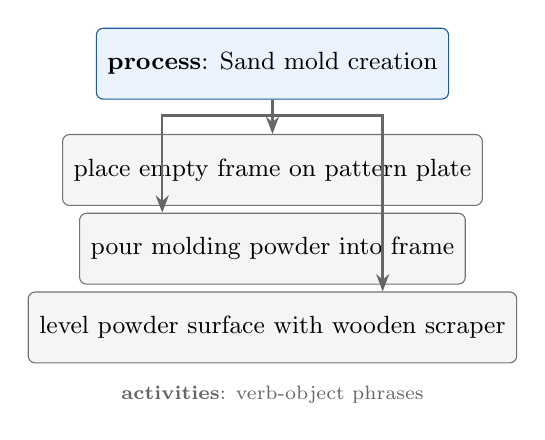
\begin{tikzpicture}[font=\small]
      \node[mmb, minimum width=40mm] (p) at (0,1.6)
        {\textbf{process}: Sand mold creation};
      \node[iob, minimum width=46mm] (a1) at (0,0.25)
        {place empty frame on pattern plate};
      \node[iob, minimum width=46mm] (a2) at (0,-0.75)
        {pour molding powder into frame};
      \node[iob, minimum width=46mm] (a3) at (0,-1.75)
        {level powder surface with wooden scraper};
      \draw[flow] (p.south) -- (a1.north);
      \draw[flow] (p.south) -- ++(0,-0.2) -| ($(a2.north)+(-1.4,0)$);
      \draw[flow] (p.south) -- ++(0,-0.2) -| ($(a3.north)+(1.4,0)$);
      \node[flab] at (0,-2.6) {\textbf{activities}: verb-object phrases};
    \end{tikzpicture}
    \end{center}
  \end{column}
  \end{columns}
\end{frame}

% ---------------------------------------------------------------- 7
\begin{frame}{From Transcript to Events}
  \begin{center}
  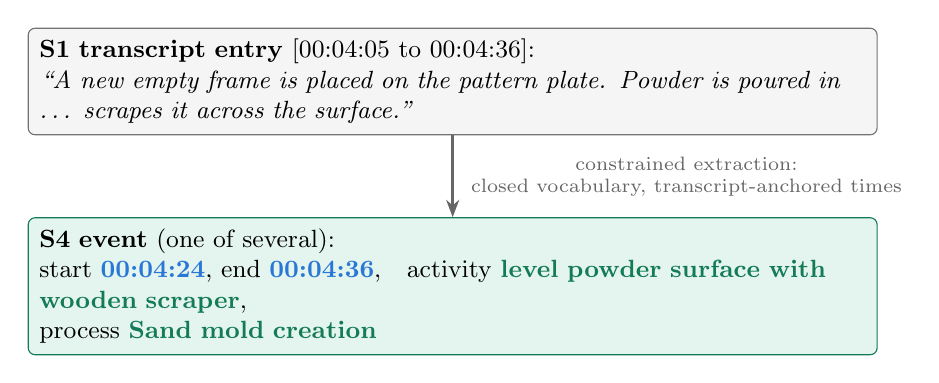
\begin{tikzpicture}[font=\small]
    \node[iob, text width=105mm, align=left] (t) at (0,0)
      {\textbf{S1 transcript entry} [00:04:05 to 00:04:36]:\\
       \emph{``A new empty frame is placed on the pattern plate.
       Powder is poured in \ldots\ scrapes it across the surface.''}};
    \node[outb, text width=105mm, align=left] (e) at (0,-2.6)
      {\textbf{S4 event} (one of several):\\
       start \keyc{00:04:24}, end \keyc{00:04:36},\quad
       activity \keyg{level powder surface with wooden scraper},\\
       process \keyg{Sand mold creation}};
    \draw[flow] (t) -- node[flab, right, xshift=1mm]
      {constrained extraction:\\closed vocabulary, transcript-anchored times}
      (e);
  \end{tikzpicture}
  \end{center}
  \vspace{2mm}
  \begin{itemize}\setlength{\itemsep}{5pt}
    \item Transcript boundaries approximate \keyc{behavioral change points}
      and become candidate \keyc{event boundaries}
    \item Non-work footage is \keya{filtered}; an empty event list is admissible
    \item Output is \keyg{schema-validated} JSON, checked against the
      vocabularies at parse time
  \end{itemize}
\end{frame}

% ---------------------------------------------------------------- 8
\begin{frame}{The Derived Dataset}
  \begin{center}
  \small
  \begin{tabular}{llrrr}
    \toprule
    Factory & Domain & Workers & Videos & Events \\
    \midrule
    001 & metal stamping and bench assembly & 11 & 97 & 2{,}288 \\
    002 & garment finishing and packaging & 10 & 54 & 1{,}541 \\
    003 & investment-casting post-processing & 11 & 72 & 2{,}449 \\
    004 & garment sewing and confection & 10 & 51 & 1{,}893 \\
    005 & machining and electric motor assembly & 11 & 22 & 1{,}103 \\
    006 & sand-casting foundry & 6 & 26 & 1{,}424 \\
    \midrule
    all & & \keyc{59} & \keyc{322} & \keyc{10{,}698} \\
    \bottomrule
  \end{tabular}
  \end{center}
  \vspace{3mm}
  \begin{itemize}\setlength{\itemsep}{5pt}
    \item Over \keyc{100 hours} of manual work, 13{,}304 transcript entries
    \item Synthetic time axis per worker (videos carry no wall-clock metadata):
      \keyg{durations and orderings} are meaningful, calendar dates are not
    \item Pipeline, prompts, logs, and assessment code \keyg{publicly released}
  \end{itemize}
\end{frame}

% ---------------------------------------------------------------- 9
\begin{frame}{Evaluation: How}
  Logs are produced by \keya{inference}, so validity comes first;
  the decisive question is \keyg{analytical value}:
  \vspace{2mm}
  \begin{itemize}\setlength{\itemsep}{8pt}
    \item \keyc{Q1 validity preconditions}: schema completeness, vocabulary
      conformance, temporal coverage, boundary alignment with the transcript,
      and a manual semantic audit
    \item \keyc{Q2 analysis capability}: four classes on the released logs:
      \keyg{time composition} (A1), \keyg{fragmentation} of value-adding work
      (A2), \keyg{control-flow discovery} (A3), \keyg{worker benchmarking} (A4)
    \item \keyc{Q3 optimization evidence}: \keyg{triangulate} the pipeline's
      own qualitative reports against the log numbers: what do event logs add
      over narrative reporting?
  \end{itemize}
  \vspace{2mm}
  \small All computations use pm4py on the released artifacts only.
\end{frame}

% ---------------------------------------------------------------- 10
\begin{frame}{Evaluation: Results}
  \begin{columns}[T]
  \begin{column}{0.5\textwidth}
    \small
    \textbf{Q1: the logs are trustworthy}
    \begin{itemize}\setlength{\itemsep}{5pt}
      \item \keyg{100\%} vocabulary conformance (10{,}698 events)
      \item Median coverage $\approx$ \keyg{95\%} for recordings up to 1 h
        (multi-hour recordings \keya{truncate} and are excluded)
      \item \keyg{82\%} of event boundaries within $\pm$5 s of a transcript
        boundary
      \item Manual audit: precision \keyg{0.86}, recall $\approx$ \keyg{0.89},
        zero contradicted labels
    \end{itemize}
  \end{column}
  \begin{column}{0.46\textwidth}
    \small
    \textbf{Q2, Q3: the logs add value}
    \begin{itemize}\setlength{\itemsep}{5pt}
      \item Non-value-adding time varies \keyc{sevenfold} across factories
        (3.7 to 25.8\%)
      \item Factory 003 spends \keya{10.8\%} of observed time
        \keya{repairing defective castings}: a cost that points upstream to
        casting quality, visible \keyg{only in the log} (no written report
        on this factory mentioned it)
      \item Interruption profiles separate \keyc{material presentation}
        from \keyc{layout and logistics} problems
      \item Benchmarking localizes spreads up to \keyc{30 points}
        on identical tasks
    \end{itemize}
  \end{column}
  \end{columns}
\end{frame}

% ---------------------------------------------------------------- 11
\begin{frame}{What Can Be Improved: Data}
  \small
  \begin{itemize}\setlength{\itemsep}{8pt}
    \item \keya{Waiting is under-measured}: the extraction keeps only
      operational events, so idle stretches rarely become events at all;
      waiting-as-waste is invisible and every reported non-value-adding share
      is therefore a \keyc{lower bound}
    \item \keya{Long recordings truncate}: extraction stops early on the seven
      multi-hour videos (median coverage 1.2\%, against about 95\% for clips
      up to one hour); \keyc{windowed extraction}, processing the transcript
      in chunks, would recover them
    \item \keya{No product identifiers}: events say what the worker does, not
      \keyg{which piece} is worked on; linking events to objects
      (\keyc{object-centric} logs) would unlock pieces per hour and
      first-pass yield
    \item \keya{Synthetic timestamps}: clips are concatenated on an artificial
      time axis, so durations and orderings are valid, but shifts, breaks, and
      utilization are not; recordings need \keyc{wall-clock anchoring}
    \item \keya{One corpus}: six factories, all discrete manufacturing;
      the \keyc{analysis classes} transfer to other domains,
      the concrete numbers do not
  \end{itemize}
\end{frame}

% ---------------------------------------------------------------- 12
\begin{frame}{What Can Be Improved: Pipeline}
  \small
  \begin{itemize}\setlength{\itemsep}{9pt}
    \item \keya{Vocabulary gaps become blind spots}. The induced vocabulary is
      the measurement instrument: what it does not name, the log cannot see.
      Factory 003 had \keya{no transport label}, so transport was transcribed
      but could not be measured.\\
      \keyc{Fix}: make a standard set of categories (transport, waiting,
      rework, inspection) \keyc{mandatory} in vocabulary induction, so an
      absent behavior is a \keyg{measured zero}, not a blind spot
    \item \keya{The video is never re-checked}. All fidelity checks compare
      events against the \keyg{transcript}, so errors made by the vision stage
      propagate silently into the logs.\\
      \keyc{Fix}: a \keyc{video-grounded audit} with several raters before any
      operational decision
    \item \keya{Results depend on prompts and model versions}. Rerunning with
      newer foundation models may change the extracted logs.\\
      \keyc{Mitigation}: \keyc{versioned prompts} and released artifacts keep
      every analysis reproducible \keyg{without model access}
  \end{itemize}
\end{frame}

% ---------------------------------------------------------------- 13
\begin{frame}{Takeaway}
  \begin{block}{}
    \centering Foundation models turn \keyc{egocentric factory video} into
    \keyg{valid, analysis-ready event logs}, with \keya{no training and no
    annotation}.
  \end{block}
  \vspace{3mm}
  \begin{itemize}\setlength{\itemsep}{7pt}
    \item 322 logs, 10{,}698 events, 6 real factories, over 100 hours of
      manual work (RQ1)
    \item Structurally sound and faithful within the dominant length regime:
      100\% vocabulary conformance, 82\% boundary alignment,
      audit precision 0.86 (RQ2)
    \item The logs \keyg{quantify}, \keyg{refine}, and \keyg{extend} what
      qualitative reports say, and expose their own \keya{vocabulary blind
      spots} (RQ3)
  \end{itemize}
  \vspace{3mm}
  \centering\small Pipeline, prompts, dataset, and assessment code:\\
  \url{https://github.com/fit-alessandro-berti/annotated-egocentric-10k-dataset}
\end{frame}

% ================================================================ appendix
\appendix

\begin{frame}
  \centering
  {\LARGE \textbf{\textcolor{egoblue}{Appendix}}}\\[3mm]
  {\large Detailed Evaluation Results}\\[5mm]
  \small All numbers from the released artifacts; recordings over one hour
  excluded from time statistics.
\end{frame}

% ---------------------------------------------------------------- A2
\begin{frame}{Appendix: Validity Preconditions (Q1)}
  \begin{center}
  \small
  \begin{tabular}{lrrrrrr}
    \toprule
    Factory & Workers & Videos & Events & Conform. & Coverage & Alignment \\
    \midrule
    001 & 11 & 97 & 2{,}288 & \keyg{100\%} & 94.8\% & 93.1\% \\
    002 & 10 & 54 & 1{,}541 & \keyg{100\%} & 28.2\% & 71.8\% \\
    003 & 11 & 72 & 2{,}449 & \keyg{100\%} & 93.0\% & 86.8\% \\
    004 & 10 & 51 & 1{,}893 & \keyg{100\%} & 92.1\% & 90.4\% \\
    005 & 11 & 22 & 1{,}103 & \keyg{100\%} & 25.0\% & 75.0\% \\
    006 &  6 & 26 & 1{,}424 & \keyg{100\%} & 14.1\% & 62.1\% \\
    \midrule
    all & 59 & 322 & 10{,}698 & \keyg{100\%} & 52.8\% & 82.1\% \\
    \bottomrule
  \end{tabular}
  \end{center}
  \vspace{2mm}
  \begin{itemize}\setlength{\itemsep}{5pt}
    \item \keyc{Conformance}: share of event labels drawn from the factory
      vocabularies; \keyc{coverage}: share of the observed span covered by
      events; \keyc{alignment}: boundaries within $\pm$5 s of a transcript
      boundary
    \item Low coverage in 002, 005, 006 stems from \keya{multi-hour recordings}
      that truncate at extraction; recordings up to one hour reach a median
      coverage of about \keyg{95\%}
  \end{itemize}
\end{frame}

% ---------------------------------------------------------------- A3
\begin{frame}{Appendix: Time Composition and Fragmentation (A1, A2)}
  \begin{columns}[T]
  \begin{column}{0.52\textwidth}
    \begin{center}
    \footnotesize
    \begin{tabular}{lrrrrrr}
      \toprule
      & VA & MH & TR & RW & Intr./h & VA run \\
      \midrule
      001 & 93.1 & 4.1 & 1.8 & 0.0 & 9.2 & 4.6 min \\
      002 & 96.3 & 0.1 & 2.3 & 0.0 & 3.9 & 8.8 min \\
      003 & 82.1 & 0.4 & 0.0 & \keya{10.8} & 3.6 & 9.0 min \\
      004 & 89.9 & 3.0 & 3.5 & 0.0 & 10.6 & 3.6 min \\
      005 & 80.6 & 5.4 & 9.7 & 0.0 & 5.6 & 6.2 min \\
      006 & 74.2 & \keya{12.1} & 7.8 & 0.0 & \keya{14.4} & \keya{3.1 min} \\
      \bottomrule
    \end{tabular}
    \end{center}
    \vspace{2mm}
    \small VA $=$ value-adding, MH $=$ material handling, TR $=$ transport,
    RW $=$ rework (\% of event-covered time); Intr./h $=$ interruptions of VA
    work per hour; VA run $=$ median uninterrupted VA stretch.
  \end{column}
  \begin{column}{0.44\textwidth}
    \begin{center}
    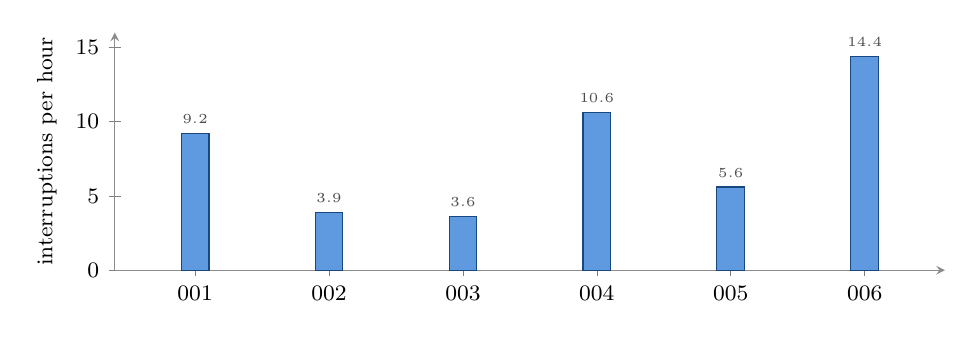
\begin{tikzpicture}
    \begin{axis}[
      ybar, bar width=10pt,
      width=\linewidth, height=4.6cm,
      ymin=0, ymax=16, ylabel={interruptions per hour},
      xtick={1,2,3,4,5,6},
      xticklabels={001,002,003,004,005,006},
      ylabel style={font=\footnotesize},
      axis lines=left, axis line style={black!45},
      enlarge x limits=0.12,
      ticklabel style={font=\footnotesize},
      nodes near coords,
      every node near coord/.append style={font=\tiny, color=black!70},
    ]
    \addplot[fill=egoblue!75, draw=egoblue!60!black]
      coordinates {(1,9.2)(2,3.9)(3,3.6)(4,10.6)(5,5.6)(6,14.4)};
    \end{axis}
    \end{tikzpicture}
    \end{center}
    \small Factory \keya{006} combines the highest interruption rate with the
    highest handling loss: a \keyc{layout and logistics} problem. Factory 001
    is interrupted often but briefly: a \keyc{material presentation} problem.
  \end{column}
  \end{columns}
\end{frame}

% ---------------------------------------------------------------- A4
\begin{frame}{Appendix: Worker Benchmarking (A4)}
  Workers on the \keyc{same dominant process} are directly comparable
  (at least 30 min of footage each):
  \vspace{1mm}
  \begin{center}
  \small
  \begin{tabular}{llrll}
    \toprule
    Factory & Shared process & Workers & VA share & Mean VA run \\
    \midrule
    001 & manual mechanical assembly & 6 & 89.7 to 97.8\% & 1.7 to 6.7 min \\
    001 & metal stamping & 3 & 90.6 to 98.5\% & 3.2 to 7.9 min \\
    003 & surface finishing and polishing & 5 & \keya{67.3 to 96.9\%} & 3.3 to 13.7 min \\
    004 & garment ironing & 2 & \keya{52.8 to 77.1\%} & 3.5 to 4.1 min \\
    004 & overlock seaming & 4 & 87.8 to 96.5\% & 1.5 to 10.3 min \\
    005 & manual lathe machining & 2 & \keyg{95.0 to 95.8\%} & 6.9 to 9.4 min \\
    \bottomrule
  \end{tabular}
  \end{center}
  \vspace{1mm}
  \small
  \begin{itemize}\setlength{\itemsep}{3pt}
    \item Large spreads (\keya{up to 30 points}) localize best practices worth
      standardizing, or hidden structural differences between stations
    \item Near-identical machinists in 005 show the opposite:
      \keyg{station design}, not behavior, drives that factory's losses
    \item Spreads are \keya{hypotheses} about stations, not verdicts on individuals
  \end{itemize}
\end{frame}

% ---------------------------------------------------------------- A5
\begin{frame}{Appendix: Triangulation Against Qualitative Reports (Q3)}
  \begin{center}
  \footnotesize
  \begin{tabular}{p{0.30\textwidth}p{0.32\textwidth}p{0.26\textwidth}}
    \toprule
    Report claim (qualitative) & Log evidence (quantitative) & Relation \\
    \midrule
    001: bottleneck is the lack of dedicated material handlers &
      14.6 handling episodes/h, mean 15 s, only 5.9\% of time &
      \keyc{Refined}: presentation, not headcount \\
    006: excessive manual handling, facility-wide bottleneck &
      19.8\% of time in handling and transport, 28.4 episodes/h &
      \keyg{Confirmed and quantified} \\
    003: workers halt work to carry heavy trays &
      transport share 0.4\%: the vocabulary has \keya{no transport label} &
      \keya{Blind spot exposed} \\
    003: report silent on rework &
      defect patching $=$ 10.8\% of observed time &
      \keyg{New, log-only finding} \\
    \bottomrule
  \end{tabular}
  \end{center}
  \vspace{2mm}
  \small Event logs \keyg{quantify} claims for prioritization,
  \keyc{refine} the intervention, surface \keyg{new findings},
  and expose what the induced vocabulary \keya{cannot see}.
\end{frame}

\end{document}
